% !TeX spellcheck = fr-toutesvariantes
\documentclass[12pt]{article}
\usepackage{longtable}
\usepackage[table,xcdraw]{xcolor}
\usepackage[utf8]{inpu	tenc}
\usepackage[T1]{fontenc}
\usepackage[francais]{babel}
\usepackage{fixltx2e}
\usepackage{charter}
\usepackage{amsmath}
\usepackage{float}
\usepackage{wrapfig}
\usepackage{graphicx}
\usepackage{soul}
\usepackage[colorlinks=true, linkcolor=blue]{hyperref}
\usepackage[a4paper, width=150mm, top=25mm, bottom=25mm]{geometry}
\usepackage{parskip}
\usepackage{enumitem}
\usepackage[final]{pdfpages}
\usepackage[linguistics]{forest}
\usepackage[final]{pdfpages}
\usepackage[font=small,labelfont=bf]{caption} % Required for specifying captions to tables and figures
\setlist[itemize]{label=\textbullet}
\usepackage[linesnumbered,algoruled,french,onelanguage]{algorithm2e}
\usepackage{url}
\usepackage{amsmath}
\usepackage{xcolor}
\usepackage{multirow}
\usepackage[noend]{algpseudocode}
\usepackage{tabularx}  % for tabularx
% to make cells in table have decent spacing
\usepackage{diagbox}
\usepackage{color, colortbl}
\usepackage{array}
\usepackage{tabularx} % in the preamble
\usepackage{csvsimple}
\usepackage{geometry}
\geometry{
	a4paper,
	total={170mm,257mm},
	left=15mm,
	top=15mm,
}
\usepackage{wrapfig}
\usepackage{multirow}
 \usepackage{booktabs}
\newcolumntype{L}[1]{>{\raggedright\let\newline\\\arraybackslash\hspace{0pt}}m{#1}}
\newcolumntype{C}[1]{>{\centering\let\newline\\\arraybackslash\hspace{0pt}}m{#1}}
\newcolumntype{R}[1]{>{\raggedleft\let\newline\\\arraybackslash\hspace{0pt}}m{#1}}

\def \hfillx {\hspace*{-\textwidth} \hfill}

\usepackage[justification=centering]{caption}
%%%%%%%%%%%%%%%%%%%%%%
\usepackage{tikz}
\usetikzlibrary{shapes.geometric, arrows}
\tikzstyle{startstop} = [rectangle, rounded corners, minimum width=3cm, minimum height=1cm,text centered, draw=black]
\tikzstyle{io} = [trapezium, trapezium left angle=70, trapezium right angle=110, minimum width=3cm, minimum height=1cm, text centered, draw=black, fill=blue!30]
\tikzstyle{process} = [rectangle, minimum width=3cm, minimum height=1cm, text centered, draw=black]
\tikzstyle{decision} = [diamond, minimum width=3cm, minimum height=1cm, text centered, draw=black, fill=green!30]

\tikzstyle{arrow} = [thick,->,>=stealth]

%%%%%%%%%%%%%%%%%%%%%%%%%



%%% Custom headers/footers (fancyhdr package)
\usepackage{fancyhdr}
\pagestyle{fancyplain}
\fancyhead{}											% No page header
\fancyfoot[L]{}											% Empty 
\fancyfoot[C]{}											% Empty
\fancyfoot[R]{\thepage}									% Pagenumbering
\renewcommand{\headrulewidth}{0pt}			% Remove header underlines
\renewcommand{\footrulewidth}{0pt}				% Remove footer underlines
\setlength{\headheight}{13.6pt}

\setlength{\parindent}{1em}

\begin{document}
\hypersetup{hidelinks}

\includepdf[pages=1]{Page_garde.pdf} 
\tableofcontents

\pagenumbering{arabic}
\newpage

%%Include Part 1
\section{Introduction}
\paragraph{}
L'objectif de ce mini-projet est de nous familiariser avec les concepts et techniques d'apprentissage automatiques supervisé (plus particulièrement les réseaux de neurones) afin de mettre en pratique ces aspects théoriques, notamment en utilisant un modèle entrainé sur un ensemble de données pour résoudre un problème en particulier.
\section{Problématique}
\paragraph{}
Dans ce projet, nous avons choisi de tenter de réaliser une application qui permettra de traduire différents gestes de la main en un texte ou une action.\par
Cette traduction automatisée peut servir par exemple à 
\begin{itemize}[label=\textbullet]
	\item Orientation à distance d'un robot.
	\item Traduction du langage des signes pour faciliter la communication avec les muets.
	\item \textbf{Air-Gesture} Communiquer une action à sa maison, son téléphone ou sa voiture avec la main ...
\end{itemize}\par 
Il devient évident que réussir à traduire(avec un taux d'exactitude assez raisonnable) des gestes de la main en temps réel(ou différé) s'avère être une tache irréalisable avec des algorithmes classiques\footnote{Algorithmes naïfs n'ayant pas recours à l'intelligence artificielle pour la résolution de problèmes}, en raison de la complexité de la relation entre les données, cela nous a donc conduits à développer un module d'apprentissage automatique basé sur les réseaux de neurones \label{ProlemSolver}
 pour accélérer l'aide à la décision, plus de détails dans \ref{neuralNetSolition}

\section{Ensemble de données}
\paragraph{}
Afin de développer le module d'apprentissage automatique mentionné dans précédemment (voir \ref{ProlemSolver}), nous avons choisit le data-set\footnote{Ensemble de données d'apprentissage} disponible dans \cite{dataset}, il s'agira donc d'analyser ces données, de les pré-traiter éventuellement afin de les préparer pour la session d'apprentissage CITER FUCKING  LEARNING HEEEEEERRE
\subsection{Description des données}
\paragraph{}
Comme expliqué dans \cite{datasetDetails}, les données d'apprentissage on été récupéré a l'aide l'application Vicon-Tracker \cite{vico} ainsi que celle de marqueurs(au total de 11) placés sur la face arrière d'un gant, ces derniers servent de source de données envoyé à des capteurs positionnés sur les deux flancs(pour calculer la profondeur), la figure suivante illustre le procédé : 
\begin{minipage}{0.5\linewidth}
	\begin{figure}[H]
		\centering
		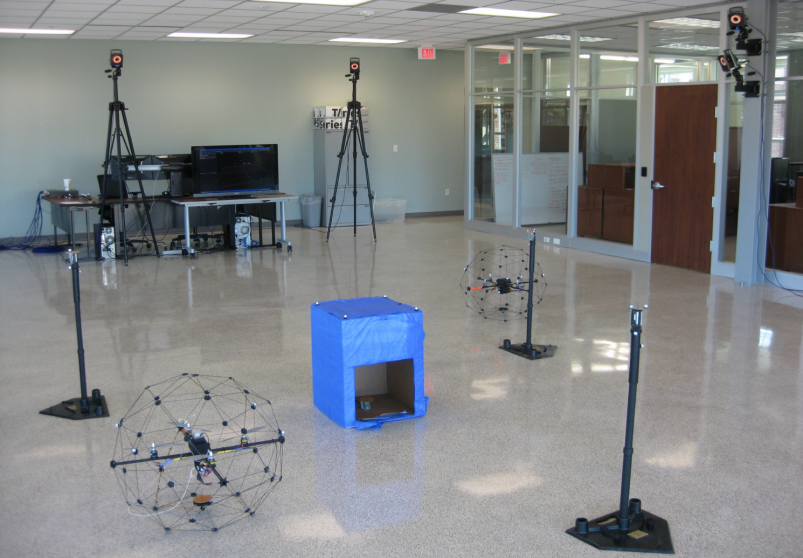
\includegraphics[width=\linewidth]{images/cameras.png}
		\caption{\small Environement ou les données on été capturées \cite{datasetDetails}}
	\end{figure}
\end{minipage}
\begin{minipage}{0.5\linewidth}
	\begin{figure}[H]
		\centering
		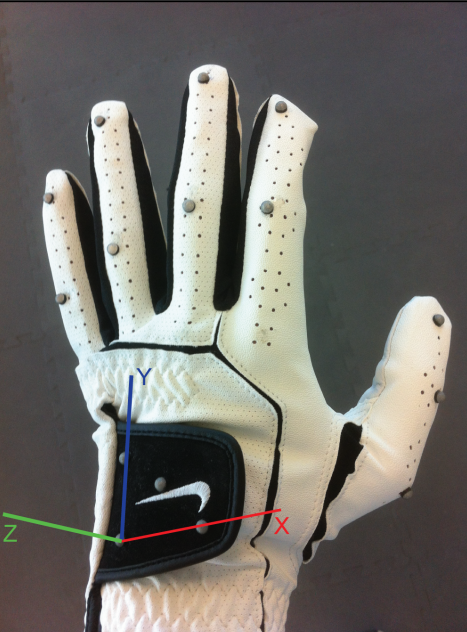
\includegraphics[width=0.5\linewidth]{images/glove.png}
		\caption{\small  Le gant utilisé pour y attaché les marqueurs( la source des données ) \cite{datasetDetails}}
	\end{figure}
\end{minipage}
\par 
Dans \cite{dataset}, on peut notamment trouvé une brève description des données brutes, elles sont sous forme d'un fichier \textbf{.csv} avec le délimiteur de cellules \textbf{,} (virgule), l'entête est structurée  de la manière suivante :
\begin{itemize}
	\item Les deux premières colonnes Class/User représentent répsectivement l'identifiant du geste observé (1 à 5) et l'identifiant de l'utilisateur(cobaye) qui a porté le gant durant cette session de collecte de données.
	\item Les 36 colonnes suivantes contiennent des nombres réels qui représentent les coordonnées cartésiennes en 3-dimensions $(x_i,y_i,z_i)$ des différents marqueurs $Marker_i$. \par Il est a noté d'après \cite{datasetDetails} et \cite{dataset} que les marqueurs sont non-étiquetés, c'est à dire que pour deux instances $I_1 et I_2$ du data-set, les coordonnés $(x_i^{I_1},y_i^{I_1},z_i^{I_1})$ et $(x_i^{I_2},y_i^{I_2},z_i^{I_2})$ ne désignent pas toujours les coordonnées du même marqueurs $i$. \par En raison des conditions de captage des données certaines instances ont des données manquantes représentées par \textbf{?}
\end{itemize}
\subsection{Analyse et prétraitement des données}
\paragraph{}
Une étape primordiale avant de se lancer dans les essaies d'apprentissage est l'analyse et la codification des données, nous avons d'abord effectué une analyse manuelle pour essayer de comprendre comment les données variaient, en nous inspirant des remarques faites dans \cite{datasetDetails} nous avons remarqué que durant l'enregistrent de la position des marqueurs, certains d'entre eux ne devenait plus visibles par les capteurs, fortement causé par la nature du geste et non pas a cause d'éventuelles perturbations, pour nous en assurer nous avons dresser le tableau suivant : 
\begin{table}[H]
	\centering
	\begin{tabular}{cc|c|c|c|c|c|c|c|c|c|}
		\cline{3-11}
		&           & \multicolumn{9}{c|}{Minimum number of Markers}                     \\ \cline{3-11} 
		& \textbf{} & 3     & 4     & 5     & 6     & 7     & 8     & 9     & 10    & 11 \\ \hline
		\multicolumn{1}{|c|}{\multirow{5}{*}{Gestures}} & 1         & 15604 & 14190 & 9191  & 2639  & 52    & 48    & 48    & 48    & 0  \\ \cline{2-11} 
		\multicolumn{1}{|c|}{}                          & 2         & 14978 & 14950 & 14909 & 14761 & 14668 & 14550 & 13524 & 10524 & 31 \\ \cline{2-11} 
		\multicolumn{1}{|c|}{}                          & 3         & 16322 & 15380 & 10746 & 6423  & 3556  & 81    & 0     & 0     & 0  \\ \cline{2-11} 
		\multicolumn{1}{|c|}{}                          & 4         & 14774 & 14769 & 14578 & 13018 & 5767  & 2349  & 13    & 0     & 0  \\ \cline{2-11} 
		\multicolumn{1}{|c|}{}                          & 5         & 15727 & 15686 & 15648 & 15406 & 14900 & 13535 & 10382 & 4180  & 0  \\ \hline
	\end{tabular}
	\caption{Nombre d'instances par classe de geste dont le nombre minimum de marqueurs est visible ( donnée non manquante dans le data-set)}
	\label{my-label}
\end{table}
\par 
Nous pouvons observer que par exemple, pour le geste 2 \textbf{tous les doigts levés} chaque instance étiquetée par cette classe possède quasiment 
tout les marqueurs visible à l'exception du dernier(puisque les marqueurs ne sont étiquetés on ne peut pas savoir le quel manque), il en est presque de même pour le geste 5 \textbf{(geste de saisie un sorte de poing ouvert légèrement)}, nous pouvons voir que qu'il y a une petite différence avec les données de la classe 2, cela est du au fait que les marqueurs placés aux ongles ne sont pas toujours visibles.\par 
Pour le reste des classes, la classe 3 et 4 diffèrent en un seul marqueurs ou deux car les deux sont très similaires( \textbf{3} : un doigt levé, \textbf{4} : deux doigts levés), enfin pour les geste de la classe 1 \textbf{(Poing fermé)} le manque apparent de marqueurs visibles est expliqué par le fait que les marqueurs au jointure et extrémité des doigts soient masqués par la nature du geste en lui même.\par 
Bien que les valeurs manquantes ont une grande signification pour nous humains, il faut tout de même traduire cette information pour le modèle, deux approches ont été pensée.
\subsubsection{Approche naïve}
\paragraph{}
Affecter une(des) valeure(s) aux données manquantes est une tâche souvent ardue, une multitude de théories existent sur le sujet, mais parfois la solution la plus simple semble être la plus efficace, nous avons simplement remplacé le valeurs manquantes par des \textbf{zeros}, ce choix est appuyé par un raisonnement fait à partir de l'analyse faite préalablement, en effet chaque classe de geste suit un certain motif(pattern) de valeurs manquantes, autrement dit si nous devions remplacer ses valeurs manquante par une approximation(une moyenne sur les valeurs de la colonne par exemple) cela pourrait rapprocher les instances entre elles et donc pourrait fausser l'apprentissage, car les valeurs des attributs seraient trop proches l'une d'entre elles, les remplacer par une valeur nulle pourra en théorie aider le modèle a mieux distinguer les classes, pour ainsi mieux approximer le pattern que suivent ces données.
\subsubsection{Approche par Clustering}
\paragraph{}
\section{Solution proposée}
\paragraph{}
Le problème ne pouvant être résolu à l'aide de techniques d'algorithmique classique(notamment à cause de sa trop forte complexité), le recours à l'apprentissage automatique s'est vu être la meilleure option.
\subsection{Apprentissage sur les données}
\paragraph{}
Après avoir analysée et traité les données, nous avons ensuite entamer la conception de notre modèle, étant donnée que nous avons utilisé deux approches pour le pré-traitement des donnés, la façon dont notre modèle va apprendre ces données pourrait différer, c'est pourquoi cette section sera diviser en deux sous-sections : \\

	\begin{tikzpicture}[node distance=2cm]
	\node (pro2a) [process, yshift=-0.5cm] {Pré-traitement des données};
	\node (pro2b) [process, below of=pro2a, xshift=-4cm] {Approche naïve};
	\node (pro2c) [process, below of=pro2a, xshift=4cm] {Approche par clustering};
	\node (pro2ca) [process, below of=pro2c,text centered, text width=3cm,minimum height=2cm] {Apprentissage \textbf{one-user-left}};
	\node (pro2ba) [process, below of=pro2b, xshift=-2cm,text centered, text width=3cm,minimum height=2cm] {Apprentissage partitionnement aléatoire};
	\node (pro2bb) [process, below of=pro2b, xshift=2cm,text centered, text width=3cm,minimum height=2cm] {Apprentissage \textbf{one-user-left}};
	\draw [arrow] (pro2a) -- (pro2b);
	\draw [arrow] (pro2a) -- (pro2c);
	\draw [arrow] (pro2b) -- (pro2ba);
	\draw [arrow] (pro2b) -- (pro2bb);
	\draw [arrow] (pro2c) -- (pro2ca);
	\end{tikzpicture}
\par 

\newpage
\section{Comparaison entre les approches}
\paragraph{}Nous commençons d'abord par donner les tableaux récapitulatifs suivants :
\paragraph{Remarques : }
\begin{itemize}
	\item Tous les essais se sont faits en 4 ré-apprentissages 
	\item chaque couche de sortie dispose de la fonction d'activation \textbf{softmax}\footnote{Fonction mathématiques de normalisation \url{https://en.wikipedia.org/wiki/Softmax_function}}, en raison de la nature de la codification choisie.
	\item La liste complète des fonctions d'apprentissages utilisées est disponible dans \cite{KerasOpt}
\end{itemize}
\begin{table}[H]
	
	\centering
	\resizebox{\textwidth}{!}{%
	\begin{tabular}{|l|c|c|c|}
		\hline
		\multicolumn{1}{|c|}{\multirow{2}{*}{Architecture}}               & \multicolumn{3}{c|}{Régression moyenne}         \\ \cline{2-4} 
		\multicolumn{1}{|c|}{}                                            & Apprentissage & Validation & Évaluation \\ \hline
		{[}40, 50, 50, 10{]} {[}'relu', 'relu', 'relu', 'relu'{]} : Nadam & 0.9719        & 0.9538     & 0.9574     \\ \hline
		{[}40, 50, 50, 20{]} {[}'relu', 'relu', 'relu', 'relu'{]} : Nadam & 0.9717        & 0.9614     & 0.9568     \\ \hline
		{[}40, 50, 50, 30{]} {[}'relu', 'relu', 'relu', 'relu'{]} : Nadam & 0.9729        & 0.95705    & 0.9559     \\ \hline
		{[}40, 50, 20{]} {[}'relu', 'relu', 'relu'{]} : Nadam             & 0.9703        & 0.9515     & 0.9550     \\ \hline
		{[}40, 50, 50, 20{]} {[}'relu', 'relu', 'relu', 'relu'{]} : Nadam & 0.9723        & 0.95113    & 0.9547     \\ \hline
	\end{tabular}
	}
	\caption{Meilleures architectures sur les données de teste pour l'approche naïve (\ref{naiveApproache}) avec partitionnement aléatoire(\ref{randomPartLearning})}
\end{table}
\paragraph{Commentaires :}\label{zeros}
La première approche(voir \ref{naiveApproache}) avec partitionnement aléatoire a  donné d'assez bons résultats, il n'y a pas eu un sur-apprentissage apparent, les instances des données de testes on été plutôt bien prédites, comme expliqué dans \ref{naiveApproache}, la discrimination a été effectuée tant bien que mal, principalement dû au motif(pattern) des valeurs manquantes qui dépend grandement des gestes de chaque utilisateur, cette approche reste encore a être testé avec des instances non-présentes dans le data-set.
\begin{table}[H]
	\centering
	\label{shit}
	\resizebox{\textwidth}{!}{%
	\begin{tabular}{|l|c|c|c|}
		\hline
		\multicolumn{1}{|c|}{\multirow{2}{*}{Architecture}}                   & \multicolumn{3}{c|}{Régression}         \\ \cline{2-4} 
		\multicolumn{1}{|c|}{}                                                & Apprentissage & Validation & Évaluation \\ \hline
		{[}40, 20{]} {[}'relu', 'relu'{]} : Adagrad  & 0.8948        & 0.8966     & 0.7918     \\ \hline
		{[}40, 20{]} {[}'relu', 'relu'{]} : Adagrad  & 0.8638        & 0.8639     & 0.7906     \\ \hline
		{[}40, 40{]} {[}'relu', 'relu'{]} : Adagrad  & 0.9057        & 0.8965     & 0.7797     \\ \hline
		{[}40, 10{]} {[}'relu', 'relu'{]} : Adadelta & 0.9396        & 0.9365     & 0.7744     \\ \hline
		{[}40, 30{]} {[}'relu', 'relu'{]} : Adagrad  & 0.8856        & 0.8827     & 0.7708     \\ \hline
	\end{tabular}
	}
	\caption{Meilleures architectures sur les données de teste pour l'approche naïve (\ref{naiveApproache}) avec partitionnement one-user-left(\ref{oneLeftLearning})}
\end{table}

\paragraph{Commentaires :	}\label{shit}
La même approche que précédemment (voir \ref{naiveApproache}) mais avec un partitionnement one-user-left, malheureusement cette approche n'a pas donné d'aussi bon résultats que la précédente, principalement dû au fait que chaque utilisateur avait une manière différente de réaliser les gestes demandés ainsi qu'au non-étiquetage des marqueurs, les données manquantes sont donc très différentes selon l'utilisateur, ainsi les données du testeur sont très mal prédites, ceci est un cas typique de sur-apprentissage.

\begin{table}[H]
	\centering
	\resizebox{\textwidth}{!}{%
	\begin{tabular}{|l|c|c|c|}
		\hline
		\multicolumn{1}{|c|}{\multirow{2}{*}{Architecture}}      & \multicolumn{3}{c|}{Régression}         \\ \cline{2-4} 
		\multicolumn{1}{|c|}{}                                   & Apprentissage & Validation & Évaluation \\ \hline
		{[}40, 20{]} {[}'relu', 'relu'{]} : Adadelta             & 0.9988        & 0.9968     & 0.9632     \\ \hline
		{[}40, 40{]} {[}'relu', 'relu'{]} : SGD                  & 0.9990        & 0.9961     & 0.9620     \\ \hline
		{[}40, 50, 10{]} {[}'relu', 'relu', 'relu'{]} : Adadelta & 0.9986        & 0.9977     & 0.9602     \\ \hline
		{[}40, 30{]} {[}'relu', 'relu'{]} : RMSprop              & 0.9982        & 0.9967     & 0.9577     \\ \hline
		{[}40, 10{]} {[}'relu', 'relu'{]} : Adam                 & 0.9983        & 0.9963     & 0.9569     \\ \hline
	\end{tabular}
	}
	\caption{Meilleures architectures sur les données de teste pour l'approche avec Clustering (\ref{clusterApproache}) avec partitionnement one-user-left(\ref{oneLeftLearning})}
\end{table}
\paragraph{Commentaires :	}
Les remarques qui sautent aux yeux sont bien entendu le très bon score à l'évaluation (meilleur que dans \ref{zeros}) ainsi que le faible écart entre données d'apprentissage, de validation et de teste, malgré un partitionnement identique à celui de \ref{shit}, la différence faite par le clustering pour le ré-étiquetage des marqueurs et la gestion des valeurs manquantes a grandement aidé à donné un pattern similaires à ces valeurs pour chaque utilisateur, cette approche a donc couvert un peu plus l'espace des données.
\section{Application dédié}
\paragraph{}
Nous avons opté à exploiter ce réseau de neurones avec une application mobile qui traduit le langage des signes en mots. L’application se connecte avec un gant qui contient des marqueurs. Ce dernier envoi à l’application les positions des marqueurs en utilisant des accéléromètres pour qu’elle puisse reconnaitre le geste effectué afin de le traduire.

Pour simuler une telle application, nous avons codé les lettres latins avec des combinaisons des cinq gestes reconnus par le réseau de neurones.\\
\begin{center}
	\begin{figure}[H]
		\centering
		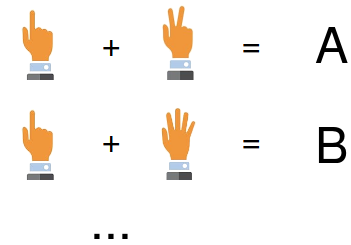
\includegraphics[scale=0.4]{images/coding.png}
		\caption{\small Codage des lettres latins en utilisant les gestes}
	\end{figure}
\end{center}
\subsection{Schéma de l’application}
\paragraph{}
L’application se devise en deux parties:
\begin{itemize}[label=\textbullet]
	\item Une pour simuler localement la traduction, c’est à dire elle utilise des données de testes déjà prêtes.
	\item L’autre recherche un gant sur le réseau, et récupère les données de ce dernier.
	Pour réaliser cette partie nous utilisons une application desktop pour simuler le gant afin d’envoyer les données à l’application. 
\end{itemize}
\begin{center}
	\begin{figure}[H]
		\centering
		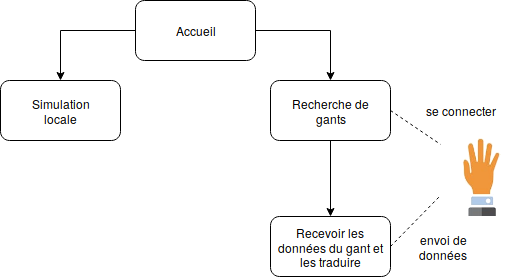
\includegraphics[scale=0.67]{images/Schema.png}
		\caption{\small Schéma générale de l’application}
	\end{figure}
\end{center}



\newpage
\listoffigures
\listoftables
\bibliographystyle{abbrv}  
\bibliography{biblio.bib}
\input{appendix.tex}
\end{document}}\grid
